\chapter{Marco de referencia}

\section{Marco Conceptual}
\label{sec:marco-conceptual}

El ajuste dinámico de la frecuencia y del voltaje para la optimización del consumo energético parte de una relación física simple entre el punto de operación elegido en el hardware, la potencia que requiere y el tiempo de ejecución. Sin embargo, su efecto depende del comportamiento de la carga, ya que una aplicación limitada por cómputo no muestra el mismo tipo de respuesta que aquella que está condicionada por el acceso a memoria. Desde esta relación se estructura el marco conceptual. En primer lugar, se expone el modelo Roofline, que permite describir ambos regímenes de ejecución; en segundo lugar, se muestran las fuentes de telemetría desde las cuales puede observarse ese comportamiento en CPU y GPU, así como los modelos ligeros que deben ser utilizados para inferirlo durante la ejecución. A partir de este punto, se expone el control DVFS desde espacio de usuario y, por último, el Producto Energía--Retardo como métrica para relacionar el ahorro energético que se obtiene dentro de la ejecución, con el efecto que la decisión genera sobre la ejecución.

El capítulo sigue esta secuencia. Las secciones \ref{sec:marco-cmos} a
\ref{sec:intensidad} presentan el fundamento físico y el criterio de
clasificación de regímenes; las secciones \ref{sec:marco-telemetria} a
\ref{sec:marco-interfaces} describen las fuentes de observación y sus
limitaciones; la sección \ref{sec:dvfs-cpu} aborda el mecanismo de actuación;
y la sección \ref{sec:marco-cargas} delimita las cargas de trabajo. Las
secciones \ref{sec:marco-ml-ligero} a
\ref{sec:marco-validacion-anidada} desarrollan el modelo de inferencia y su
evaluación, mientras que las secciones
\ref{sec:marco-pruebas-estadisticas} y \ref{sec:marco-edp} establecen los
criterios para valorar experimentalmente el sistema propuesto.

\subsection{Termodinámica del silicio y potencia CMOS}
\label{sec:marco-cmos}

La disipación de potencia en un circuito CMOS moderno se descompone en potencia estática (corrientes de fuga) y potencia dinámica, originada por la conmutación de cargas capacitivas. Como DVFS actúa sobre frecuencia y voltaje, su efecto principal recae sobre la potencia dinámica, modelable para una compuerta como:

\begin{equation}
P_{\text{dyn}} = \alpha \cdot C \cdot V^{2} \cdot f
\end{equation}

donde $\alpha$ es el factor de actividad, $C$ la capacitancia efectiva conmutada y $V$, $f$ el voltaje y la frecuencia de operación \cite{Gonzalez1997}. Dado que operar a mayor frecuencia suele exigir mayor voltaje por integridad temporal, reducir frecuencia habitualmente permite también reducir voltaje, con una caída de potencia más que proporcional por la dependencia cuadrática en $V$. Este acoplamiento es la base física del compromiso energía--rendimiento en DVFS: cuánto se gana en potencia al bajar el punto operativo depende del comportamiento computacional predominante de la aplicación, no solo de la reducción de frecuencia en sí.

\subsection{Modelo Roofline y regímenes de limitación del rendimiento}
\label{sec:roofline}

El modelo Roofline relaciona el rendimiento alcanzable de una carga con su
intensidad operacional y con los límites de cómputo y ancho de banda de la
plataforma:

\begin{equation}
P = \min\left(P_{\text{pico}},\; I \cdot BW_{\text{pico}}\right)
\label{eq:roofline}
\end{equation}

donde $P_{\text{pico}}$ representa el rendimiento aritmético pico, $I$ la
intensidad operacional, expresada como operaciones por byte transferido desde
memoria, y $BW_{\text{pico}}$ el ancho de banda pico
\cite{Williams2009}. Cuando el límite viene dado por
$I \cdot BW_{\text{pico}}$, la carga se encuentra en régimen
\textit{memory-bound}; cuando corresponde a $P_{\text{pico}}$, se encuentra
en régimen \textit{compute-bound}.

\begin{figure}[H]
    \centering
    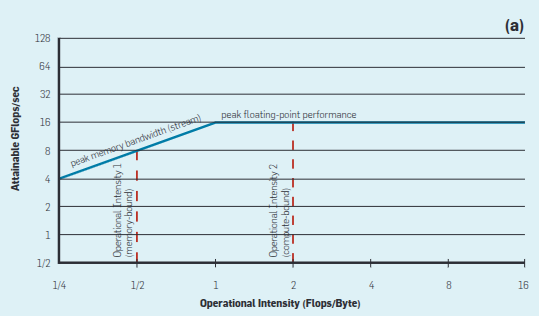
\includegraphics[width=0.72\textwidth]
        {figuras/fig_modelo_roofline_conceptual_williams2009.png}
    \caption[Modelo Roofline conceptual]{Modelo Roofline conceptual y relación entre el techo de ancho de banda de memoria y el techo de rendimiento de cómputo. Tomado de Williams et al. \cite[Fig.~1(a)]{Williams2009}.}
    \label{fig:modelo-roofline-conceptual}
\end{figure}

La intensidad operacional relaciona el trabajo aritmético con los bytes
transferidos desde el nivel de memoria analizado y no con el tamaño nominal del
conjunto de trabajo \cite[p.~66]{Williams2009}. Una carga que excede la
capacidad de la caché no es necesariamente \textit{memory-bound}, ya que la
reutilización de datos puede reducir el tráfico hacia memoria y aumentar su
intensidad operacional \cite[Secs.~3--4]{Goto2008}.

\subsubsection{Punto de inflexión y criterio de clasificación}
\label{sec:marco-ridge}

La frontera entre ambos regímenes corresponde al punto de inflexión o
\textit{ridge point}, donde las dos ramas de \eqref{eq:roofline} se igualan:

\begin{equation}
I_{\text{ridge}} =
\frac{P_{\text{pico}}}{BW_{\text{pico}}}
\label{eq:ridge}
\end{equation}

En este trabajo, $I_{\text{ridge}}$ define el criterio de etiquetado. Una
intensidad inferior se clasifica como \textit{memory-bound} y una superior
como \textit{compute-bound} \cite{Williams2009}. Como el techo de cómputo
depende de la precisión aritmética, cada precisión requiere su propio
$I_{\text{ridge}}$ \cite{Antepara2025}. Las cargas de precisión mixta
requieren, por ello, un tratamiento específico antes de compararse con un
único techo.

El punto de inflexión también cambia con la frecuencia. El rendimiento pico de
cómputo y el ancho de banda de memoria pertenecen a dominios distintos y no
varían necesariamente en la misma proporción
\cite{Guerreiro2019,Ali2023}. Por esta razón, $I_{\text{ridge}}$ debe
calibrarse para cada precisión y nivel de frecuencia, evitando atribuir a la
carga un cambio originado por el punto operativo.

Los valores nominales del hardware sirven como referencia, pero los techos
empleados para la clasificación deben obtenerse mediante calibración empírica
bajo las condiciones del experimento \cite{NERSC2026}.

\subsubsection{Cálculo de la intensidad operacional observada}
\label{sec:intensidad}

La intensidad operacional observada durante un intervalo $i$ se calcula como:

\begin{equation}
I_i =
\frac{\text{FLOPs}_i}{B_i^{\text{DRAM}}}
\label{eq:intensidad}
\end{equation}

donde $\text{FLOPs}_i$ representa el trabajo aritmético realizado y
$B_i^{\text{DRAM}}$ los bytes transferidos hacia o desde memoria principal
durante el mismo intervalo \cite{Williams2009}. Ambas magnitudes deben
corresponder a los mismos límites temporales. Combinar mediciones con
granularidades distintas produciría una intensidad sin consistencia física
(sección \ref{sec:ventanas}).

En CPU, los FLOPs se obtienen mediante eventos de la PMU cuya codificación y
semántica dependen de la microarquitectura \cite{Weaver2008}. El tráfico de
memoria se mide mediante los contadores \textit{uncore} del controlador de
memoria integrado, descritos en la sección \ref{sec:uncore}. Cuando estos
operan con una granularidad más gruesa que los contadores de núcleo, los FLOPs
se agregan sobre el mismo intervalo antes de calcular la intensidad
operacional.

\subsection{Telemetría microarquitectónica}
\label{sec:marco-telemetria}

Los procesadores modernos incorporan Unidades de Monitorización de Rendimiento
(\textit{Performance Monitoring Units}, PMU), que permiten observar mediante
hardware eventos asociados a la ejecución. Entre ellos se encuentran las
instrucciones retiradas, los ciclos de procesador, los fallos de caché y otros
eventos definidos por la microarquitectura. Algunos contadores están asociados
a eventos fijos y otros pueden programarse mediante la codificación establecida
por el fabricante \cite{IntelSDM2026}.

Esta capacidad de observación está limitada por el número de contadores físicos
disponibles. Cuando se solicitan más eventos de los que pueden medirse
simultáneamente, el kernel puede multiplexarlos y estimar los conteos a partir
del tiempo durante el cual cada evento estuvo habilitado y efectivamente activo
\cite{Liu2024}. La estimación pierde precisión cuando la tasa del evento cambia
durante los intervalos no observados. Por esta razón, el conjunto de eventos
debe mantenerse dentro de la capacidad de la PMU y las lecturas utilizadas en
el análisis deben verificarse mediante \textit{time running} y
\textit{time enabled} \cite{Liu2024,LinuxPerfEventOpen2026}.

Los eventos también difieren en la forma como se solicitan, por ejemplo, Linux proporciona
eventos genéricos que el kernel traduce a la plataforma disponible, mientras
que los eventos crudos utilizan directamente la codificación definida por la
microarquitectura \cite{Weaver2015,IntelSDM2026}. Estos últimos permiten acceder
a señales que no disponen de una abstracción genérica, pero requieren comprobar
que el código, la máscara y los calificadores correspondan al procesador
evaluado. La apertura correcta del contador no basta para garantizar que el
valor obtenido tenga la interpretación esperada.

\subsubsection{Contadores de núcleo y contadores de \textit{uncore}}
\label{sec:uncore}

Las señales necesarias para caracterizar una carga no proceden de un único
dominio del procesador. Los contadores de núcleo observan eventos asociados a
la ejecución sobre uno o varios núcleos y pueden vincularse con un proceso. Los
contadores de \textit{uncore} cubren recursos compartidos del zócalo, entre
ellos el controlador de memoria, la caché de último nivel y las
interconexiones, por lo que sus mediciones tienen alcance de sistema.

Esta diferencia es especialmente relevante para la intensidad operacional
definida en la sección \ref{sec:intensidad}. El trabajo aritmético puede
obtenerse mediante eventos asociados a la ejecución de la carga, mientras que
el tráfico hacia memoria principal se observa mediante los contadores del
controlador de memoria integrado. Estos contabilizan transferencias que
alcanzan la DRAM, incluidos accesos de demanda y precarga
\cite{IntelUncore2021}, y proporcionan los bytes utilizados en el denominador
de la intensidad operacional. Su alcance compartido también implica
restricciones de acceso distintas a las de los contadores de núcleo, descritas
en la sección \ref{sec:marco-interfaces}.


\begin{figure}[H]
\centering

\begin{tikzpicture}[
font=\small,
box/.style={
draw,
rounded corners,
align=center,
minimum height=1cm,
minimum width=4.4cm
},
arrow/.style={
-{Latex[length=2mm]},
thick
}
]

% Entrada
\node[align=center] (events)
{Eventos\\microarquitectónicos};

% Contadores
\node[box, right=2.2cm of events, yshift=1.25cm] (fixed)
{\textbf{Contadores fijos}\\
FC$_0$, FC$_1$, \ldots\\
eventos predefinidos\\
(instrucciones, ciclos)};

\node[box, below=0.8cm of fixed] (programmable)
{\textbf{Contadores programables}\\
PMC$_0$, PMC$_1$, \ldots, PMC$_n$};

% Configuración
\node[box, below=0.8cm of programmable] (control)
{\textbf{Registros de configuración}\\
\textit{Event Select} + \textit{Unit Mask}\\
+ calificadores};

% Marco de PMU
\node[
draw,
rounded corners,
fit=(fixed)(programmable)(control),
inner sep=0.35cm,
label=above:\textbf{PMU}
] (pmu) {};

% Flechas
\draw[arrow] (events.east) -- ++(0.75,0)
|- (fixed.west);

\draw[arrow] (events.east) -- ++(0.75,0)
|- (programmable.west);

\draw[arrow] (control.north) -- (programmable.south);

\end{tikzpicture}

\caption[Unidad de Monitorización de Rendimiento (PMU)]{Organización conceptual de una Unidad de Monitorización de
Rendimiento (PMU) con contadores fijos y programables.
Fuente: elaboración propia.}
\label{fig:pmu-conceptual}
\end{figure}

\subsubsection{Métricas microarquitectónicas de eficiencia}
\label{sec:marco-metricas-eficiencia}

Los contadores de rendimiento permiten derivar señales que describen distintos
aspectos de la ejecución. El IPC relaciona las instrucciones retiradas con los
ciclos transcurridos y permite observar el aprovechamiento del procesador
\cite[Ch.~6]{Gregg2020}, por otra parte, los eventos \texttt{cache-references} y
\texttt{cache-misses} permiten calcular la tasa de fallos de caché y el MPKI,
dos medidas de presión sobre la jerarquía de memoria.Al ser eventos genéricos, su implementación depende del la microarquitectura y no
asegura la medición de un nivel específico de caché \cite{LinuxPerfEventOpen2026}.

Los ciclos de estancamiento aportan información sobre intervalos en los que la
ejecución deja de progresar al ritmo esperado. Un contador agregado del
\textit{backend} no permite determinar si la espera procede de memoria o de
otros recursos internos \cite{VTune2026}, debido a esto, para aproximar con mayor precisión
las esperas relacionadas con memoria pueden emplearse eventos específicos que
contabilizan ciclos con solicitudes de carga pendientes
\cite{IntelPerfmon2026}. Como ocurre con los demás eventos crudos, su uso
requiere verificar previamente la codificación y la semántica definidas para
la microarquitectura \cite{Weaver2008,IntelSDM2026}.

En resumen,el IPC,fallos de caché y ciclos de estancamiento se utilizan como señales
observables del comportamiento de la carga. Ninguna de ellas determina por sí
sola si una ejecución pertenece al régimen \textit{compute-bound} o
\textit{memory-bound}. Esa etiqueta procede del criterio Roofline definido a
partir de la intensidad operacional y del punto de inflexión de la plataforma
\cite{Williams2009}. Las métricas microarquitectónicas cumplen una función
distinta y sirven como características a partir de las cuales el clasificador
intenta inferir dicho régimen.

\subsubsection{Ventanas de muestreo y naturaleza temporal de la observación}
\label{sec:ventanas}

Las lecturas de los contadores representan valores acumulados desde su
activacion o último reinicio \cite{LinuxPerfEventOpen2026}. Las métricas de
cada ventana se obtienen, por ello, mediante la diferencia entre dos lecturas
consecutivas y utilizando el tiempo realmente transcurrido entre ambas. Este
intervalo debe medirse con una fuente temporal que no cambie ante ajustes del
reloj del sistema \cite{LinuxClockGettime2026}.

El período de muestreo determina la resolución con la que pueden observarse
cambios en la carga. Reducirlo mejora la resolución temporal, pero aumenta la
frecuencia de lectura y la sobrecarga asociada
\cite{LinuxPerfStat2026}. Además, no todas las fuentes de telemetría operan con
la misma granularidad. Cuando los contadores de \textit{uncore} producen
intervalos más amplios que los contadores de núcleo, las magnitudes utilizadas
para calcular la intensidad operacional deben agregarse sobre un intervalo
común antes de aplicar el criterio Roofline.

\subsection{Espacios de ejecución: \textit{user-space} y \textit{kernel-space}}
\label{sec:marco-espacios-ejecucion}

El sistema operativo restringe el acceso directo a sus recursos mediante la
separación entre modo usuario y modo kernel \cite[ch.~2]{Kerrisk2010}. Las
operaciones de control de memoria, entrada/salida y manejo de dispositivos
permanecen bajo control del núcleo, por lo que las aplicaciones ordinarias se
comunican con el hardware mediante las interfaces que este expone
\cite{McCarty2015}.

En este trabajo, el servicio de control se ejecuta en espacio de usuario para
evitar la complejidad de compilar e insertar un módulo dentro del kernel de
Linux. Esta decisión obliga a realizar el monitoreo de la carga y los ajustes
de frecuencia mediante interfaces provistas por el sistema operativo, con el
costo temporal asociado a esas operaciones frente a un control ejecutado
directamente dentro del kernel.

\begin{figure}[H]
\centering
\begin{tikzpicture}[
    every node/.style={font=\small},
    app/.style={rectangle, draw=green!45!black, fill=white,
        minimum width=2.2cm, minimum height=0.90cm, align=center, rounded corners=1pt},
    kmod/.style={rectangle, draw=blue!45!black, fill=white,
        minimum width=2.3cm, minimum height=0.95cm, align=center, rounded corners=1pt},
    zoneuser/.style={rectangle, draw=green!45!black, thick, fill=green!12,
        rounded corners=2pt, inner xsep=0.4cm, inner ysep=0.4cm},
    zonekernel/.style={rectangle, draw=blue!45!black, thick, fill=blue!8,
        rounded corners=2pt, inner xsep=0.4cm, inner ysep=0.4cm},
    hw/.style={rectangle, draw=black!55, thick, fill=black!8,
        minimum width=6.4cm, minimum height=1.05cm, align=center, rounded corners=2pt},
    arr/.style={-{Stealth[length=2mm]}, thick}
]
    \node[app] (app1) {Aplicación 1};
    \node[app, right=0.5cm of app1] (app2) {Aplicación 2};
    \node[font=\large, right=0.4cm of app2] (dots1) {$\cdots$};
    \node[app, right=0.4cm of dots1] (appn) {Aplicación N};
    \coordinate (uhead) at ($(app1.north)+(0,0.85)$);

    \node[kmod, below=3.4cm of app1] (proc) {Gestión de\\procesos};
    \node[kmod, right=0.4cm of proc] (mem) {Gestión de\\memoria};
    \node[kmod, right=0.4cm of mem] (fs) {Sistema de\\archivos};
    \node[kmod, right=0.4cm of fs] (drv) {Controladores\\de dispositivos};
    \node[font=\large, right=0.3cm of drv] (dots2) {$\cdots$};
    \coordinate (khead) at ($(proc.north)+(0,0.85)$);

    \begin{pgfonlayer}{background}
        % Se elimina la etiqueta 'label=above:...' para que no dibuje fuera del recuadro
        \node[zoneuser, fit=(app1)(app2)(dots1)(appn)(uhead)] (userzone) {};
        \node[zonekernel, fit=(proc)(mem)(fs)(drv)(dots2)(khead)] (kernelzone) {};
        \node[fit=(userzone)(kernelzone), inner sep=0pt] (span) {};
    \end{pgfonlayer}

    % Títulos internos de USER SPACE
    \node[font=\bfseries] at ([yshift=-0.28cm]userzone.north) {USER SPACE};
    \node[font=\small] at ([yshift=-0.80cm]userzone.north) {(Espacio de usuario)};

    % Títulos internos de KERNEL SPACE
    \node[font=\bfseries] at ([yshift=-0.28cm]kernelzone.north) {KERNEL SPACE};
    \node[font=\small] at ([yshift=-0.80cm]kernelzone.north) {(Espacio del kernel)};

    \coordinate (boundaryY) at ($(userzone.south)!0.5!(kernelzone.north)$);
    \draw[dashed, thick] (span.west |- boundaryY) -- (span.east |- boundaryY);
    \node[font=\small, align=left, anchor=west]
        at ($(span.east |- boundaryY)+(0.3,0)$)
        {Interfaz de\\llamadas al sistema\\(límite)};

    \draw[arr] (app1.south) -- (app1.south |- kernelzone.north);
    \draw[arr] (appn.south |- kernelzone.north) -- (appn.south);

    \node[hw, below=1.2cm of kernelzone] (hardware) {\textbf{HARDWARE}\\\small(Hardware físico)};
    \draw[{Stealth[length=2mm]}-{Stealth[length=2mm]}, thick] (kernelzone.south) -- (hardware.north);
\end{tikzpicture}
\caption[Espacios de usuario y de kernel]{Relación conceptual entre \textit{user-space}, \textit{kernel-space} y el hardware físico, mediada por la interfaz de llamadas al sistema. Fuente: elaboración propia.}
\label{fig:user-kernel-space}
\end{figure}

\subsection{Interfaces estándar de observabilidad e instrumentación}
\label{sec:marco-interfaces}

El agente requiere obtener señales de CPU y GPU desde espacio de usuario sin
modificar el kernel ni los controladores. En Linux, esta observación puede
realizarse mediante \texttt{perf\_event} para los contadores de rendimiento,
Intel RAPL para energía de CPU y NVIDIA Management Library (NVML) para el
estado operativo de la GPU
\cite{Weaver2015,David2010,NVML2026}. Estas interfaces constituyen las fuentes
de telemetría utilizadas por el proyecto y determinan qué información puede
observarse durante la ejecución.

\subsubsection{La interfaz \texttt{perf\_event}}
\label{sec:perfevent}

Linux expone \texttt{perf\_event} para acceder desde espacio de usuario a los
eventos registrados por la PMU \cite{LinuxPerfEventOpen2026}. La interfaz
permite observar instrucciones, ciclos y otros eventos microarquitectónicos
sin acceder directamente a los registros del procesador. También permite
asociar la medición a una tarea o realizarla sobre recursos de alcance más
amplio, diferencia que condiciona qué actividad contribuye a cada conteo.

En este trabajo, \texttt{perf\_event} proporciona las señales de núcleo
utilizadas para caracterizar la ejecución en CPU y da acceso a los eventos
específicos requeridos por el instrumento. Los contadores de
\textit{uncore}, en cambio, observan recursos compartidos y requieren un
alcance distinto al de una medición atribuible únicamente al proceso. Esta
diferencia explica por qué las señales de núcleo y el tráfico de memoria
descrito en la sección \ref{sec:uncore} no comparten necesariamente el mismo
ámbito de observación.

El acceso a estos contadores está sujeto a las restricciones que Linux impone
sobre la monitorización de rendimiento mediante
\texttt{perf\_event\_paranoid} y los privilegios asociados
\cite{LinuxPerfEventOpen2026}. Para el proyecto, esta restricción determina
qué eventos pueden obtenerse desde espacio de usuario y cuáles requieren
permisos adicionales. La configuración concreta de esos permisos forma parte
del procedimiento experimental y se describe posteriormente en la metodología.

\subsubsection{Intel RAPL}
\label{sec:rapl}

Intel RAPL (\textit{Running Average Power Limit}) es un mecanismo de
monitorización y gestión energética integrado en procesadores Intel. La
plataforma expone contadores acumulativos asociados a distintos dominios de
energía, cuya disponibilidad depende de la microarquitectura
\cite{David2010,Thamm2025}. Entre ellos puede encontrarse el dominio
\textit{Package}, que representa el consumo energético del conjunto del
procesador dentro del zócalo, y el dominio DRAM, asociado a la memoria cuando
el hardware dispone de esta medición.

La energía consumida durante un intervalo se obtiene a partir de la diferencia
entre dos lecturas consecutivas de estos contadores, debido a que estas presentan desbordamiento durante ejecuciones prolongadas. En este trabajo, RAPL se
utiliza para medir la energía de CPU y relacionarla con el tiempo de ejecución
durante la evaluación de las decisiones DVFS. La medición queda restringida a
los dominios que el procesador expone mediante RAPL y, por tanto, no representa
el consumo eléctrico completo del nodo \cite{Thamm2025}.

\subsubsection{NVIDIA Management Library y Nsight Compute}
\label{sec:marco-nvml-ncu}

NVIDIA Management Library (NVML) es una interfaz de programación proporcionada
por NVIDIA para consultar desde espacio de usuario el estado operativo de la
GPU. Entre las métricas disponibles se encuentran la utilización del
dispositivo, la actividad de memoria, la potencia y las frecuencias de
operación \cite{NVML2026}. Estas señales describen el comportamiento agregado
del acelerador durante la ejecución y pueden obtenerse sin instrumentar los
kernels de la aplicación.

El nivel de observación de NVML no permite reconstruir directamente la
intensidad operacional del modelo Roofline. La utilización indica actividad
del dispositivo, pero no cuantifica por sí misma las operaciones de punto
flotante ejecutadas ni los bytes transferidos hacia la memoria global. En este
trabajo, sus métricas se emplean como señales observables para el clasificador
de GPU, mientras que la etiqueta de régimen se obtiene mediante una
caracterización independiente.

NVIDIA Nsight Compute es un perfilador de kernels CUDA que proporciona
información más detallada sobre la ejecución, incluidos conteos relacionados
con operaciones aritméticas, instrucciones y tráfico de memoria
\cite{Nsight2026}. Esta información permite estimar la intensidad operacional
de cada carga y ubicarla respecto al punto de inflexión de la plataforma. El
perfilado puede requerir varias pasadas sobre un mismo kernel para recolectar
todas las métricas solicitadas, lo que incrementa su costo y limita su uso como
fuente de observación durante la ejecución.


\subsection{Gestión dinámica de frecuencia en sistemas operativos
mediante DVFS, P-states y \textit{governors}}
\label{sec:dvfs-cpu}

El escalado dinámico de voltaje y frecuencia
(\textit{Dynamic Voltage and Frequency Scaling}, DVFS) permite modificar el
punto operativo del procesador para ajustar su capacidad de cómputo y su
consumo energético \cite{Hebbar2022}. En CPU, el hardware dispone de varios
niveles de rendimiento que pueden seleccionarse mientras el procesador
permanece activo. Dentro del modelo ACPI, estos niveles se representan mediante
P-states y proporcionan la base sobre la cual el sistema operativo solicita
cambios de rendimiento.

La disponibilidad de varios estados requiere una política que determine cuál
solicitar durante la ejecución. Linux organiza este control mediante el
subsistema CPUFreq, donde los \textit{governors} aplican distintos criterios
de selección y el controlador de frecuencia comunica la solicitud al mecanismo
soportado por el procesador \cite{Hebbar2022,LinuxCPUFreq2026}. La elección del
nivel y su aplicación sobre el hardware corresponden, por tanto, a funciones
diferentes dentro del control DVFS.

Los \textit{governors} nativos utilizan reglas propias para seleccionar el
nivel de rendimiento. \texttt{performance} y \texttt{powersave} operan sobre
los extremos del rango disponible, mientras que \texttt{ondemand},
\texttt{conservative} y \texttt{schedutil} ajustan la solicitud durante la
ejecución \cite{Hebbar2022,LinuxCPUFreq2026}. Estas políticas sirven como
referencia para evaluar el agente propuesto, cuya decisión de frecuencia se
basa en el régimen de ejecución inferido por el clasificador y se aplica
mediante la infraestructura de control disponible en Linux.

La solicitud emitida por la política no determina necesariamente el reloj que
alcanza físicamente el procesador. Controladores como
\texttt{intel\_pstate} pueden delegar parte de la gestión al propio hardware
mediante \textit{Hardware-Managed P-states} (HWP)
\cite{LinuxIntelPstate2026,Hebbar2022}. El valor solicitado debe interpretarse
entonces como una petición de rendimiento cuyo resultado depende también del
mecanismo que gobierna el punto operativo.

La autonomía del hardware también interviene cuando está habilitado Turbo
Boost. Este mecanismo puede modificar la frecuencia según las condiciones
térmicas, eléctricas y de utilización del procesador
\cite{LinuxIntelPstate2026,Hebbar2022}. Dos niveles solicitados pueden producir
relojes efectivos similares si estas condiciones permiten al hardware operar
fuera del valor esperado. Por esta razón, una comparación entre niveles DVFS
requiere comprobar la frecuencia alcanzada bajo carga en lugar de asumirla a
partir del valor solicitado.

La diferencia entre solicitud y frecuencia efectiva introduce además una
restricción temporal. El nuevo punto operativo requiere un intervalo para
materializarse y su tiempo de respuesta depende de la plataforma y del
mecanismo utilizado \cite{Hebbar2022}. La frecuencia solo puede emplearse como
acción de control si el cambio llega a establecerse dentro de la escala
temporal en la que se toman las decisiones.

\subsubsection{Dominios de frecuencia y topología SMT}
\label{sec:dominios}

La frecuencia efectiva también depende del alcance físico de la política sobre
la que se realiza la solicitud. CPUFreq asocia cada política con uno o varios
procesadores lógicos, cuya agrupación depende del hardware y del controlador
activo \cite{LinuxCPUFreq2026}. La CPU lógica donde se fija una carga no
representa necesariamente un dominio de frecuencia independiente.

Esta condición resulta especialmente relevante cuando está habilitado
\textit{simultaneous multithreading} (SMT). Dos procesadores lógicos hermanos
comparten un mismo núcleo físico y sus solicitudes de rendimiento pueden
influir sobre la frecuencia alcanzada por ese núcleo
\cite{LinuxIntelPstate2026}. Fijar la ejecución a uno de los hermanos controla
la afinidad de la carga, pero no aísla por sí solo el estado de frecuencia del
núcleo compartido.

La afinidad y el control de frecuencia deben considerarse entonces como
propiedades distintas del experimento. Cuando se modifica el punto operativo
de una carga, deben tenerse en cuenta los procesadores lógicos asociados al
mismo núcleo y comprobarse la frecuencia alcanzada después de la solicitud.
Esta verificación permite relacionar los cambios de tiempo y energía con el
estado realmente aplicado por el hardware.

\begin{figure}[H]
    \centering
    \begin{tikzpicture}[
        font=\small,
        cpu/.style={
            draw,
            rounded corners,
            minimum width=3cm,
            minimum height=1cm,
            align=center
        },
        request/.style={
            draw,
            rounded corners,
            minimum width=2.6cm,
            minimum height=0.9cm,
            align=center
        },
        arrow/.style={
            -{Latex[length=2mm]},
            thick
        }
    ]

    \node[cpu] (cpu0)
        {CPU lógica A\\\footnotesize ejecuta la carga};

    \node[cpu, right=2.2cm of cpu0] (cpu1)
        {CPU lógica B\\\footnotesize hermano SMT};

    \node[
        draw,
        rounded corners,
        fit=(cpu0)(cpu1),
        inner sep=0.5cm,
        label=above:\textbf{Núcleo físico compartido}
    ] (core) {};

    \node[request, below=1.3cm of cpu0] (req0)
        {Límite solicitado\\$f_{\mathrm{baja}}$};

    \node[request, below=1.3cm of cpu1] (req1)
        {Solicitud del hermano\\$f_{\mathrm{alta}}$};

    \draw[arrow] (req0.north) -- (cpu0.south);
    \draw[arrow] (req1.north) -- (cpu1.south);

    \node[fit=(req0)(req1), inner sep=0pt] (requests) {};

    \node[
        draw,
        rounded corners,
        minimum width=4.5cm,
        minimum height=1cm,
        align=center,
        below=0.9cm of requests
    ] (effective)
        {\textbf{Frecuencia efectiva del núcleo}\\
        condicionada por ambas solicitudes};

    \draw[arrow] (core.south) -- (effective.north);

    \end{tikzpicture}

    \caption[Solicitudes de frecuencia entre hermanos SMT]
    {Relación entre las solicitudes de rendimiento de dos procesadores
    lógicos hermanos y la frecuencia efectiva del núcleo físico compartido.
    Nota. Elaboración propia con base en la documentación de
    \texttt{intel\_pstate} \cite{LinuxIntelPstate2026}.}
    \label{fig:smt-frecuencia}
\end{figure}

\subsubsection{Particularidades de DVFS en GPU}
\label{sec:dvfs-gpu}

En GPU, el efecto de un cambio de frecuencia depende del recurso que limita la
ejecución. El dispositivo dispone de un dominio de procesamiento, asociado
principalmente a los multiprocesadores de \textit{streaming} (SM), y de un
dominio de memoria vinculado al movimiento de datos hacia la memoria del
dispositivo \cite{Guerreiro2019,Ali2023}. La influencia de cada dominio cambia
según el comportamiento de la carga.

Esta dependencia se relaciona con los regímenes definidos mediante Roofline.
Cuando una carga es \textit{compute-bound}, el rendimiento está más ligado a
la capacidad de los SM y una modificación de su frecuencia puede producir un
cambio apreciable en el tiempo de ejecución. En una carga
\textit{memory-bound}, el movimiento de datos adquiere mayor peso y la
sensibilidad al reloj de procesamiento puede disminuir
\cite{Guerreiro2019,Ali2023}. El régimen inferido proporciona así información
para decidir cuánto puede afectar una modificación del reloj de procesamiento
al rendimiento de la carga.

\begin{figure}[H]
    \centering
    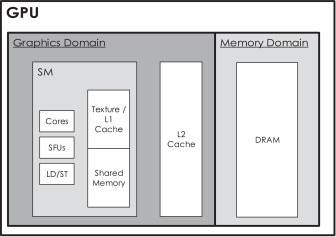
\includegraphics[width=0.58\textwidth]
        {figuras/fig_dominios_gpu_guerreiro_2019.jpg}
    \caption[Dominios de procesamiento y memoria en GPU]
    {Dominios de procesamiento y memoria considerados en una GPU.
    Nota. Adaptado de Guerreiro et al. \cite{Guerreiro2019}.}
    \label{fig:dominios-gpu}
\end{figure}

El efecto sobre el tiempo debe evaluarse junto con el consumo energético.
Reducir el reloj de procesamiento puede disminuir la potencia instantánea y
prolongar al mismo tiempo la ejecución \cite{Ali2023}. La energía consumida
depende de ambos efectos, por lo que una frecuencia menor no implica por sí
sola una mejora. Esta relación justifica evaluar las decisiones DVFS mediante
una métrica que considere conjuntamente energía y tiempo, como el EDP empleado
posteriormente en el trabajo.

La transición hacia otro nivel de frecuencia introduce además un tiempo de
respuesta propio del acelerador. La solicitud emitida desde el host debe ser
aplicada por el dispositivo y el nuevo reloj necesita un intervalo para
alcanzar un estado estable. Esta latencia depende de la arquitectura y del par
de frecuencias involucrado \cite{Velicka2025}, por lo que debe conocerse antes
de establecer la permanencia mínima de una decisión.

Una transición comparable con la duración del intervalo sobre el que se
pretende actuar puede consumir una parte importante del tiempo disponible para
aprovechar el nuevo punto operativo. La política de control debe considerar,
por esta razón, tanto el régimen inferido como el tiempo requerido para
materializar el cambio. Si ese costo temporal no puede amortizarse, modificar
la frecuencia deja de ser una acción útil aunque la clasificación del régimen
sea correcta.

\subsection{Cargas de trabajo mediante kernels, benchmarks y microbenchmarks}
\label{sec:marco-cargas}

Las aplicaciones de cómputo de alto rendimiento pueden presentar regiones con
demandas distintas de cómputo y memoria, por lo que una medida agregada de toda
la ejecución puede ocultar esos cambios de comportamiento. Para estudiar esta
variación se emplean kernels, entendidos como unidades de trabajo con un patrón
computacional delimitado, como una multiplicación de matrices o una
transformada de Fourier \cite{Williams2009}. En este trabajo, esta delimitación
permite relacionar la telemetría observada con la intensidad operacional y con
el régimen de ejecución determinado mediante Roofline.

Los kernels utilizados para construir esa caracterización proceden de
benchmarks reproducibles que representan distintos patrones algorítmicos y de
acceso a memoria \cite[Ch.~12]{Gregg2020}. Su función no es aportar de antemano
una clase de rendimiento, sino proporcionar cargas suficientemente diversas
para observar cómo responde la plataforma ante comportamientos distintos. La
clasificación como \textit{memory-bound} o \textit{compute-bound} se obtiene a
partir de la intensidad operacional medida respecto al punto de inflexión
calibrado, por lo que el nombre o la procedencia del benchmark no determinan la
etiqueta utilizada por el clasificador.

Los microbenchmarks se utilizan con un propósito diferente. Estas cargas
reducen la ejecución a una operación controlada para medir propiedades
concretas de la plataforma, como el ancho de banda de memoria o la capacidad
aritmética \cite[Ch.~12]{Gregg2020}. En este trabajo, esas mediciones se
emplean para obtener los límites de cómputo y memoria necesarios para calibrar
el modelo Roofline y calcular el punto de inflexión. Los microbenchmarks de
calibración cumplen así una función de referencia de la plataforma y no
sustituyen las cargas empleadas para construir el conjunto de entrenamiento.
\subsection{Aprendizaje automático supervisado ligero}
\label{sec:marco-ml-ligero}

La clasificación del régimen de ejecución se plantea como un problema
supervisado en el que las señales observadas durante la ejecución se relacionan
con una etiqueta conocida durante el entrenamiento
\cite[Ch.~2]{James2021}. Para este trabajo, el modelo debe distinguir entre
\textit{compute-bound} y \textit{memory-bound} utilizando únicamente
información que pueda obtenerse durante la operación del sistema. Las
magnitudes empleadas para construir la etiqueta Roofline quedan fuera de las
entradas del clasificador, ya que su inclusión reproduciría el criterio de
etiquetado en lugar de inferirlo a partir de la telemetría disponible.

La predicción forma parte del mismo ciclo en el que se observa la carga y se
decide sobre la frecuencia. Su costo temporal debe ser pequeño frente al
intervalo disponible para actuar, de modo que una mejora en clasificación no
quede anulada por el tiempo necesario para obtenerla. El término
\textit{ligero} se utiliza con este criterio y depende de la complejidad del
modelo finalmente entrenado, no únicamente de la familia a la que pertenece.
La selección considera por ello el desempeño predictivo junto con la latencia
de una predicción individual.

\subsubsection{Familias de modelos candidatas}
\label{sec:marco-familias-modelos}

La comparación parte de modelos simples y avanza hacia alternativas capaces de
representar relaciones no lineales entre las señales de entrada. Este rango
permite determinar si el problema requiere la complejidad de un ensamble o si
una estructura más sencilla ofrece una clasificación suficiente con menor
costo de inferencia.

\paragraph{Regresión logística.}

La regresión logística proporciona una referencia lineal para la separación de
las clases \cite[Ch.~4]{James2021}. Su inferencia requiere pocas operaciones,
por lo que sirve para establecer cuánto puede resolverse a partir de una
relación lineal entre las características observadas. La comparación con los
modelos posteriores muestra si incorporar relaciones no lineales aporta una
mejora relevante para el problema.

\paragraph{Árbol de decisión.}

Los árboles de decisión separan las observaciones mediante reglas sucesivas
sobre las características de entrada \cite[Ch.~8]{James2021}. Esta forma de
particionar los datos admite relaciones no lineales sin requerir la evaluación
de múltiples modelos durante una predicción. Las reglas obtenidas también
pueden inspeccionarse directamente, lo que facilita identificar qué señales
intervienen en la separación entre los dos regímenes.

\paragraph{Bosques aleatorios.}

Random Forest combina varios árboles cuyas diferencias se introducen durante
el entrenamiento mediante muestreo y selección aleatoria de características
\cite{Breiman2001}. La decisión final integra las predicciones de esos árboles,
lo que puede reducir la dependencia de una partición particular de los datos.
A cambio, una inferencia requiere recorrer varios estimadores. Su comparación
con un árbol individual permite medir si la mejora predictiva obtenida
compensa ese costo adicional.

\paragraph{Árboles extremadamente aleatorizados.}

Extra-Trees mantiene el uso de múltiples árboles, pero añade aleatoriedad a los
puntos de corte considerados durante su construcción
\cite{Geurts2006}. La diferencia respecto a Random Forest modifica la forma en
que el ensamble divide el espacio de características y ofrece una segunda
alternativa basada en árboles múltiples. Su evaluación permite comprobar si
esa estrategia mejora la clasificación manteniendo una latencia compatible
con la inferencia durante la ejecución.

\paragraph{XGBoost.}

XGBoost construye un ensamble de árboles de manera secuencial y utiliza cada
nueva etapa para corregir parte del error acumulado por el modelo
\cite{Chen2016}. Esta capacidad permite representar interacciones más complejas
entre características, aunque la inferencia depende del número de árboles y de
su profundidad. Se incorpora como una referencia de mayor capacidad para
determinar si una mejora predictiva justifica utilizar un modelo más costoso.

Las familias consideradas cubren así distintos niveles de complejidad sin
establecer una preferencia previa por alguna de ellas. La elección del modelo
depende de cuánto mejora la clasificación y del tiempo necesario para producir
cada predicción. Un aumento de complejidad solo resulta útil para el servicio
de control cuando la ganancia predictiva compensa el costo adicional de
inferencia.

\subsection{Evaluación del desempeño de un clasificador}
\label{sec:marco-evaluacion-clasificador}

La evaluación de un clasificador parte de la matriz de confusión, que
relaciona las clases reales con las predicciones del modelo. En el caso
binario, sus resultados se expresan mediante verdaderos positivos ($TP$),
verdaderos negativos ($TN$), falsos positivos ($FP$) y falsos negativos
($FN$). Estas cantidades permiten examinar el desempeño global y el
comportamiento del modelo sobre cada clase \cite{SokolovaLapalme2009}.

La exactitud (\textit{accuracy}) mide la proporción de predicciones
correctas:

\begin{equation}
    \mathrm{Accuracy}
    =
    \frac{TP+TN}{TP+TN+FP+FN}.
\end{equation}

Su interpretación requiere considerar la distribución de las clases, ya que
un conjunto desbalanceado puede producir una exactitud elevada aun cuando el
modelo tenga un desempeño deficiente sobre la clase menos representada
\cite{Brodersen2010}. Por esta razón, la evaluación se complementa con
métricas calculadas para cada clase.

La precisión y la sensibilidad se definen como:

\begin{equation}
    \mathrm{Precision}
    =
    \frac{TP}{TP+FP},
    \qquad
    \mathrm{Recall}
    =
    \frac{TP}{TP+FN}.
\end{equation}

El puntaje $F_1$ combina ambas medidas mediante su media armónica:

\begin{equation}
    F_1
    =
    2
    \frac{
        \mathrm{Precision}\,\mathrm{Recall}
    }{
        \mathrm{Precision}+\mathrm{Recall}
    }.
\end{equation}

Como estas métricas dependen de la clase considerada positiva, su valor debe
examinarse para cada clase. Cuando se requiere un único valor de resumen, el
$F_1$ macro asigna el mismo peso a ambas clases:

\begin{equation}
    F_{1,\mathrm{macro}}
    =
    \frac{F_{1,1}+F_{1,2}}{2}.
\end{equation}

Este promedio evita que la clase más frecuente determine por sí sola la
medida global y permite conservar una lectura equilibrada del desempeño del
clasificador \cite{SokolovaLapalme2009}.

\subsubsection{Línea base de referencia}
\label{sec:marco-lineas-base}

Las métricas del clasificador adquieren mayor significado cuando se comparan
con una referencia que no utiliza las características de entrada. Una línea
base sencilla consiste en predecir siempre la clase mayoritaria, cuyo resultado
representa el desempeño que puede obtenerse únicamente a partir de la
distribución de las etiquetas, sin explotar la telemetría utilizada por el
modelo.

La comparación con esta referencia permite determinar si las características
aportan capacidad discriminativa bajo el protocolo de evaluación empleado, por lo cual, si el modelo no supera la línea base, los resultados no proporcionan evidencia
suficiente de una mejora predictiva atribuible a las variables utilizadas.

\subsubsection{Costo de inferencia}
\label{sec:marco-costo-inferencia}

En un clasificador destinado a operar dentro de un sistema de control en
línea, la calidad predictiva debe evaluarse junto con el tiempo requerido para
obtener cada decisión, teniendo esto en cuenta,la magnitud de interés es la latencia de una predicción
individual, ya que el modelo procesa un vector de características por cada
evento de decisión.

La latencia presenta variación entre predicciones, por lo que una medida
central no describe por completo su comportamiento. Su caracterización puede
complementarse con percentiles altos, como p95 y p99, que permiten observar la
cola de la distribución \cite{Georges2007}, por lo que la viabilidad temporal del modelo
depende de que estas latencias sean compatibles con el presupuesto disponible
para la decisión del agente. De esta forma, la selección del clasificador
considera conjuntamente su capacidad predictiva y el costo temporal de
ejecutar la inferencia.

\subsection{Optimización de hiperparámetros y Optuna}
\label{sec:marco-optuna}

El comportamiento de un modelo no depende únicamente del algoritmo empleado,
sino también de los hiperparámetros que determinan aspectos como la
profundidad de un árbol, el número de estimadores de un ensamble o la
intensidad de la regularización. Estos valores no se obtienen durante el
ajuste de los parámetros internos del modelo, por lo que deben seleccionarse
mediante un proceso de búsqueda sobre distintas configuraciones
\cite{Bergstra2012}.

Optuna organiza esta búsqueda mediante ensayos sucesivos, denominados
\textit{trials}, estos ensayos evalúan una combinación de hiperparámetros a
partir de una función objetivo, mientras que los resultados obtenidos quedan
disponibles para orientar las evaluaciones siguientes. La exploración deja
así de depender de recorrer de forma exhaustiva todas las combinaciones
posibles y puede concentrarse progresivamente en zonas del espacio de búsqueda
que han producido mejores valores de la función objetivo
\cite{Akiba2019}.

Entre las estrategias que pueden emplearse en este proceso se encuentra el
\textit{Tree-structured Parzen Estimator} (TPE). Este método utiliza los
ensayos ya evaluados para distinguir configuraciones asociadas con mejores y
peores resultados y, a partir de esa distribución, proponer nuevos valores.
La búsqueda conserva cierta exploración del espacio disponible, pero dedica
una mayor parte de las evaluaciones a regiones que muestran mayor potencial
de mejora.

La selección de hiperparámetros también afecta la forma en que debe estimarse
el desempeño del modelo. Cuando los mismos datos intervienen tanto en la
elección de la configuración como en su evaluación final, el resultado puede
quedar favorecido por el propio proceso de búsqueda. La validación anidada
evita esta superposición al separar la selección interna de hiperparámetros de
la evaluación utilizada para estimar la capacidad de generalización
\cite{Cawley2010}.

La validez de esa evaluación depende además de que las características de
entrada no revelen información contenida en la variable objetivo o en el
procedimiento utilizado para construirla. Cuando esto ocurre, el modelo puede
apoyarse en información que no estaría disponible en las condiciones reales
de predicción, produciendo fuga de información \cite{Kaufman2012}. En estos casos, la partición debe conservar juntas las
observaciones relacionadas \cite{Roberts2017}.

\subsection{Comparaciones estadísticas pareadas}
\label{sec:marco-pruebas-estadisticas}

Cuando dos condiciones se evalúan sobre las mismas unidades experimentales,
las observaciones correspondientes forman pares y no deben tratarse como
muestras independientes. El análisis se realiza entonces sobre las diferencias
observadas para cada unidad, permitiendo evaluar si existe un efecto sistemático
asociado a la condición comparada \cite[Ch.~2]{Montgomery2017}.

La prueba $t$ pareada contrasta si la media de estas diferencias es
estadísticamente distinguible de cero y supone una distribución aproximadamente
normal de las diferencias. Cuando este supuesto no resulta adecuado, la prueba
de rangos con signo de Wilcoxon constituye una alternativa no paramétrica que
utiliza el signo y el orden de las diferencias en lugar de depender
directamente de sus magnitudes \cite[Ch.~3]{Hollander2014}. El valor $p$
obtenido mediante una prueba de hipótesis permite cuantificar la evidencia
contra la ausencia de una diferencia sistemática, pero no expresa por sí mismo
la magnitud del efecto observado.

El remuestreo \textit{bootstrap} permite complementar este análisis mediante
la estimación de intervalos de confianza para el estadístico de interés. A
partir de remuestreos con reemplazo de las observaciones disponibles se obtiene
una distribución empírica que permite caracterizar la incertidumbre asociada
al efecto estimado sin imponer una distribución paramétrica específica
\cite[Chs.~12--14]{EfronTibshirani1993}.

La capacidad para detectar una diferencia depende del número de observaciones
y de su variabilidad. Por esta razón, un resultado no significativo indica
falta de evidencia suficiente para rechazar la hipótesis nula, pero no demuestra
que las condiciones comparadas sean equivalentes.

\subsection{Producto Energía--Retardo (EDP)}
\label{sec:marco-edp}

La evaluación de una estrategia de gestión energética debe considerar
conjuntamente el consumo de energía y el tiempo de ejecución, ya que una
reducción de potencia puede acompañarse de un incremento temporal suficiente
para anular el beneficio energético. El Producto Energía--Retardo
(\textit{Energy--Delay Product}, EDP) combina ambas magnitudes en una única
métrica \cite{Laros2013}:

\begin{equation}
    EDP = E \cdot T,
\end{equation}

donde $E$ corresponde a la energía consumida y $T$ al tiempo de ejecución.
Un menor valor de EDP representa un compromiso más favorable entre ambas
magnitudes bajo este criterio.

La formulación admite una generalización que pondera explícitamente el peso
relativo del tiempo frente a la energía:

\begin{equation}
    \mathrm{ED}^{n}\mathrm{P} = E \cdot T^{n},
    \label{eq:ednp}
\end{equation}

donde $n$ expresa cuánto se penaliza la degradación temporal. Con $n=1$ se
recupera el EDP, mientras que $n=2$ define el ED$^{2}$P, empleado cuando el
rendimiento debe preservarse con mayor prioridad que el consumo
\cite{Laros2013,Ali2023}. La elección de $n$ es una decisión del evaluador y no
una propiedad del sistema medido: dos valores distintos pueden ordenar de forma
diferente las mismas configuraciones, por lo que debe declararse explícitamente
antes de comparar resultados.

El EDP resulta especialmente útil en la evaluación de técnicas DVFS, donde la
reducción de frecuencia puede disminuir la potencia instantánea pero aumentar
el tiempo de ejecución. Por ello, evaluar únicamente potencia, energía o
rendimiento de forma aislada puede conducir a conclusiones distintas de las
obtenidas al considerar conjuntamente el costo energético y temporal
\cite{Ali2023,Laros2013}.

\subsection{Síntesis: alcance y límites del marco adoptado}
\label{sec:marco-sintesis}

Los conceptos anteriores convergen en un compromiso metodológico concreto. La
etiqueta de régimen procede del modelo Roofline y exige una medida directa de
trabajo aritmético y de tráfico hacia memoria principal, disponible fuera de
línea pero costosa o inaccesible durante la ejecución. Las señales que sí
pueden leerse con baja intrusión describen actividad y no intensidad
operacional, de modo que el clasificador se define precisamente como el
sustituto que traduce las segundas en la primera. Esta separación entre la
fuente de la verdad y la fuente de la predicción es la decisión de diseño
central del trabajo, y de ella se desprenden las salvaguardas desarrolladas en
las secciones previas: la exclusión de la magnitud que origina la etiqueta del
vector de entrada, la partición por unidad experimental y no por observación
individual, y la comparación contra líneas base sin capacidad predictiva.

Este marco delimita también lo que el trabajo no puede afirmar. La
clasificación es binaria y estática respecto a un umbral calibrado, por lo que
no describe fases intermedias ni transiciones continuas entre regímenes. La
observabilidad disponible es asimétrica entre dispositivos, de manera que la
misma pregunta no admite el mismo grado de evidencia en CPU y en GPU. Y el
mecanismo de actuación tiene un costo temporal propio que acota la granularidad
útil de cualquier política, con independencia de la calidad del clasificador.
En consecuencia, un resultado que no muestre mejora sobre las líneas base o
sobre los gobernadores nativos no invalidaría el marco: sería la respuesta que
este marco permite dar sobre los límites de la telemetría y del mecanismo de
control disponibles en la plataforma evaluada.


\section{Estado del Arte}
\label{sec:estado-del-arte}

La gestión energética en sistemas de alto rendimiento ha evolucionado desde enfoques estáticos de reducción de potencia hacia estrategias cada vez más adaptativas, orientadas a preservar el rendimiento sin incurrir en costos energéticos desproporcionados. Dentro de este proceso, el escalado dinámico de voltaje y frecuencia (DVFS) se ha consolidado como uno de los mecanismos más estudiados para modificar el punto operativo de procesadores y aceleradores. Su aplicación, sin embargo, no conduce necesariamente al mismo resultado para todas las cargas de trabajo. La reducción de frecuencia puede disminuir la potencia instantánea, pero también prolongar el tiempo de ejecución y anular el beneficio energético esperado. Por esta razón, una parte importante de la investigación en este campo se ha desplazado desde la aplicación uniforme de DVFS hacia mecanismos capaces de reconocer el comportamiento de la carga y seleccionar configuraciones acordes con sus características.

Una de las primeras evidencias de esta dependencia fue presentada por Calore et al. \cite{Calore2017}, quienes estudiaron el efecto de DVFS sobre una CPU Intel Haswell y una GPU NVIDIA K80 mediante distintos kernels y una aplicación HPC completa. Los autores analizaron conjuntamente el tiempo y la energía de ejecución, y mostraron que una misma frecuencia no resulta igualmente conveniente para todas las regiones de una aplicación. En lugar de mantener un único estado operativo durante toda la ejecución, evaluaron cambios de frecuencia a nivel de función, lo que permitió observar que las oportunidades de ahorro dependen tanto de la naturaleza de la región ejecutada como de la arquitectura sobre la cual se realiza el cálculo. Este resultado introduce una idea central para los mecanismos de gestión adaptativa: la decisión de frecuencia debe responder al comportamiento de la carga y no únicamente a una política global fijada de antemano.

Aunque esta aproximación permite aprovechar diferencias entre regiones de ejecución, requiere conocimiento previo sobre la estructura de la aplicación y puntos específicos en los cuales realizar la actuación. El problema se desplaza entonces hacia la posibilidad de caracterizar automáticamente una carga a partir de información observable durante su ejecución. En este sentido, Guerreiro et al. \cite{Guerreiro2019} estudiaron la relación entre el comportamiento de aplicaciones GPGPU y las variaciones de frecuencia de los dominios de cómputo y memoria. Su propuesta parte de métricas recolectadas en una configuración inicial y utiliza esa caracterización para anticipar la respuesta de la aplicación frente a otras configuraciones DVFS. De esta manera, los autores reducen la necesidad de recorrer exhaustivamente el espacio de frecuencias y muestran que es posible utilizar información de rendimiento para agrupar aplicaciones según su sensibilidad a DVFS y seleccionar configuraciones energéticamente favorables.

La propuesta de Guerreiro et al. \cite{Guerreiro2019} resulta particularmente significativa porque introduce la clasificación como un mecanismo intermedio entre la observación de la carga y la decisión energética. No obstante, las clases definidas en su trabajo responden principalmente a la sensibilidad de las aplicaciones frente a modificaciones en las frecuencias de cómputo y memoria, y no a una detección continua de fases \textit{compute-bound} y \textit{memory-bound} durante la ejecución. Su objetivo consiste en utilizar una caracterización limitada para inferir el comportamiento esperado bajo distintas configuraciones, manteniendo además el análisis concentrado en GPU. Aun así, el estudio demuestra que las métricas obtenidas del hardware contienen información suficiente para reducir el espacio de búsqueda de una configuración energética adecuada.

La misma problemática de evitar una exploración exhaustiva fue abordada posteriormente por Ali et al. \cite{Ali2023}. Los autores propusieron un método automatizado y portable para seleccionar frecuencias de GPU a partir de métricas obtenidas inicialmente en la configuración predeterminada del dispositivo. Sobre esta caracterización construyen modelos de potencia y tiempo de ejecución, con los cuales estiman la respuesta de la aplicación en otros estados DVFS sin necesidad de ejecutarla en cada uno de ellos. La selección final se realiza considerando simultáneamente consumo energético y degradación del desempeño, de modo que una reducción de potencia no sea interpretada automáticamente como una mejora si viene acompañada de un incremento excesivo en el tiempo de ejecución. En las plataformas evaluadas, la propuesta alcanzó reducciones promedio de energía de 29.6\% con una pérdida de rendimiento de 5.2\% sobre NVIDIA GA100 y de 22.6\% con una pérdida de 4.7\% sobre NVIDIA GV100 \cite{Ali2023}.

En conjunto, los trabajos de Guerreiro et al. \cite{Guerreiro2019} y Ali et al. \cite{Ali2023} muestran que el espacio DVFS puede reducirse mediante modelos construidos a partir del comportamiento de la aplicación. Sin embargo, ambos enfoques parten principalmente de una caracterización utilizada para predecir configuraciones posteriores. Esta estrategia es adecuada cuando la aplicación puede tratarse como una carga relativamente estable, pero resulta más limitada cuando su comportamiento cambia durante la ejecución. Las aplicaciones científicas suelen combinar regiones con demandas diferentes sobre las unidades de cómputo y el subsistema de memoria; por tanto, una política verdaderamente adaptativa requiere no solo estimar qué frecuencia puede resultar adecuada, sino también reconocer cuándo cambia el régimen de ejecución.

La clasificación de este comportamiento constituye precisamente el problema abordado por Antici et al. \cite{Antici2024} mediante MCBound. Los autores plantean la distinción entre cargas \textit{memory-bound} y \textit{compute-bound} como un problema de clasificación basado en datos, utilizando información de ejecuciones HPC para caracterizar automáticamente nuevos trabajos. Su evaluación sobre datos del supercomputador Fugaku mostró que esta separación puede realizarse con una puntuación F1-macro de al menos 0.89 y con un costo reducido para el funcionamiento del sistema \cite{Antici2024}. Este resultado aporta evidencia directa de que la naturaleza computacional de una carga puede inferirse automáticamente en lugar de depender exclusivamente de una clasificación manual basada en el conocimiento previo de la aplicación.

MCBound representa un antecedente especialmente cercano al componente de clasificación, aunque su propósito no es gobernar directamente los estados DVFS de CPU o GPU. La clasificación se utiliza para caracterizar trabajos HPC, pero no se integra con un mecanismo que traduzca de manera continua la clase inferida en una decisión de frecuencia durante las distintas fases de la ejecución. Esta separación resulta importante: demostrar que una carga puede clasificarse como limitada por memoria o por cómputo resuelve el problema de identificación, pero aún queda por determinar cómo utilizar esa información dentro de una política energética y si el costo de realizar dicha inferencia es suficientemente bajo para justificar su uso en tiempo de ejecución.

La actuación dinámica sobre la frecuencia dentro de una aplicación científica ha sido explorada por Simsek et al. \cite{Simsek2024} en el contexto de simulaciones astrofísicas ejecutadas sobre GPU. Los autores instrumentaron SPH-EXA para medir el comportamiento energético de diferentes regiones y modificar la frecuencia del acelerador en puntos determinados de la ejecución. Frente a una política de frecuencia uniforme, esta adaptación permitió reducir el consumo energético por GPU hasta en 7.82\%, con una degradación del rendimiento de aproximadamente 2.95\%. El estudio demuestra que existe un beneficio potencial al cambiar la frecuencia durante la ejecución y no únicamente antes de iniciar la aplicación. No obstante, la decisión depende de la instrumentación del código y del conocimiento de las regiones sobre las cuales se debe actuar, por lo que la política permanece vinculada a la estructura particular de la aplicación \cite{Simsek2024}.

Un antecedente adicional, más cercano a un control \textit{online} completo, es DRLCAP, un marco de \textit{frequency capping} de GPU en tiempo de ejecución basado en aprendizaje por refuerzo profundo. DRLCAP monitoriza información a nivel de sistema para detectar cambios de fase y ajustar el límite de frecuencia sin intervención manual, reduciendo en promedio 22\% de la energía de GPU con menos de 3\% de degradación de rendimiento en arquitecturas NVIDIA \cite{Wang2024}. Este resultado confirma que el control \textit{online} de frecuencia es factible y efectivo, pero también expone una diferencia de diseño relevante para este trabajo: la política se aprende mediante refuerzo profundo, orientada exclusivamente a GPU, en lugar de formularse como una clasificación supervisada ligera de fases seguida de una decisión discreta e interpretable, coordinada sobre CPU y GPU.

Los antecedentes revisados permiten observar una evolución clara del problema. Calore et al. \cite{Calore2017} mostraron que diferentes regiones de una aplicación pueden requerir configuraciones DVFS distintas; Guerreiro et al. \cite{Guerreiro2019} demostraron que la sensibilidad a la frecuencia puede caracterizarse a partir de métricas de ejecución; Ali et al. \cite{Ali2023} utilizaron esta idea para estimar configuraciones energéticamente convenientes sin recorrer todo el espacio DVFS; Antici et al. \cite{Antici2024} evidenciaron que la distinción entre cargas \textit{compute-bound} y \textit{memory-bound} puede plantearse como un problema de clasificación; Simsek et al. \cite{Simsek2024} comprobaron que modificar dinámicamente la frecuencia dentro de una aplicación científica puede producir ahorros energéticos medibles; y Wang et al. \cite{Wang2024} demostraron con DRLCAP que un controlador \textit{online} aprendido puede gobernar la frecuencia de GPU en tiempo real con resultados energéticos favorables. En conjunto, estos trabajos cubren las principales etapas necesarias para construir un mecanismo de gestión adaptativa, aunque dichas etapas aparecen generalmente resueltas de manera independiente.

A partir de esta revisión, el problema de investigación no radica en demostrar nuevamente que DVFS puede disminuir el consumo energético ni en establecer que las cargas pueden clasificarse de acuerdo con su comportamiento. La cuestión que permanece abierta para el presente trabajo es cómo integrar ambas capacidades dentro de un mecanismo de control de baja intrusión que pueda operar durante la ejecución. En particular, interesa determinar si la telemetría disponible desde espacio de usuario permite alimentar un clasificador supervisado ligero que identifique el régimen predominante de la carga y utilice esa información como señal para aplicar una política DVFS previamente caracterizada sobre el hardware.

Finalmente, la revisión evidencia una concentración importante de los enfoques recientes de predicción y selección de frecuencia en GPU. Aunque Calore et al. \cite{Calore2017} consideran conjuntamente CPU y GPU, los trabajos de Guerreiro et al. \cite{Guerreiro2019}, Ali et al. \cite{Ali2023}, Simsek et al. \cite{Simsek2024} y Wang et al. \cite{Wang2024} profundizan principalmente en aceleradores gráficos. Esta diferencia es relevante para un entorno heterogéneo, ya que CPU y GPU no ofrecen las mismas fuentes de telemetría, poseen mecanismos distintos de gestión de frecuencia y pueden responder de manera diferente ante una reducción del reloj. Por esta razón, una estrategia de control para sistemas CPU--GPU debe reconocer dichas diferencias en lugar de aplicar una única regla de observación y actuación a ambos dispositivos. El propósito del presente trabajo se sitúa precisamente en esta integración: utilizar mecanismos de clasificación de bajo costo como señal de contexto para decisiones DVFS y evaluar empíricamente si dicha estrategia mejora el compromiso entre energía y rendimiento frente a los mecanismos nativos de gestión de frecuencia.
